\section{Sicurezza Informatica}

\subsection{Salvare password nel Database}%
\label{sub:password}

Per permettere la persistenza delle prenotazioni e per garantire la non repudiabilit\`a delle informazioni, ogni utente dovr\`a registrarsi con email e password e utilizzare l'account per la maggior parte delle operazione nel Servizio. Per rispettare gli standard di sicurezza non \`e possibile salvare la password degli utenti nel database ma \`e necessario crittografarla. Le funzioni di Hash sono funzioni a una sola direzione che permettono di derivare una sequenza di byte deterministica a partire da una stringa fornita in input. Queste funzioni possono essere utilizzate per derivare un dato che permetta di verificare la correttezza di una password senza aver bisogno di salvare la password in chiaro. Quando l'utente si registra verr\`a salvata nel database la password crittografata da un algoritmo, al successivo accesso da parte dell'utente la password fornita verr\`a crittografata utilizzando lo stesso algoritmo e poi verr\`a confrontata con la stringa di byte salvata nel database. Se i due dati sono identici la password \`e la stessa di quella di registrazione e l'accesso viene autorizzato.

Gli algoritmi di hashing non sono abbastanza da soli per proteggere una password, \`e necessario concatenare una stringa casuale chiamata \emph{salt} alla password prima di usare l'algoritmo di hashing e l'output della funzione di hash deve essere ripetutamente passato alla funzione di hash, pi\`u volte viene ripetuto questo processo e pi\`u difficile sar\`a ottenere la password dal risultato. Si consiglia di ripetere il procedimento un minimo di 10000 volte. Questo algoritmo \`e stato implementato nella funzione di hash chiamata \emph{bcrypt}. Il salt dovr\`a essere salvato in un database separato da quello degli hash (serve per impedire di riconoscere le password duplicate nel database in caso di data breach).

\subsection{Autenticazione delle richieste}%
\label{sub:authentication}

Autenticare le richieste in un sito web statico non \`e semplice. La pagina d'accesso non user\`a un form comune ma invier\`a una richiesta tramite Javascript alle API che genereranno un token che identifica univocamente l'utente. Il token ha una scadenza, ad una scadenza breve corrisponde una sicurezza maggiore perci\`o viene spesso impostato a una decina di minuti, al termine della scadenza il token viene invalidato e sar\`a necessario richiederne un altro. Questo token viene chiamato \emph{Access Token} e insieme ad esso il server durante l'autenticazione ci comunicher\`a anche un token ausiliario chiamato \emph{Refresh Token}. Il \emph{Refresh Token} permette di richiedere un nuovo \emph{Access Token} in qualsiasi momento, il client Javascript si occupa di gestire la scadenza e di chiedere un nuovo token prima poco prima della scadenza del precedente. Anche il \emph{Refresh Token} ha una scadenza ma pu\`o essere molto pi\`u lunga siccome non viene comunicato a nessun altro oltre che all'\emph{Authentication Server} (mentre l'\emph{Access Token} viene condiviso con i servizi del sito web).

I token vengono salvati nello storage locale del browser, altre informazioni sono solitamente salvate insieme ai token quali il nome utente e informazioni generiche del profilo.

Ogni richiesta che richiede l'autenticazione sar\`a inviata con l'header \emph{Authentication} contenente l'\emph{Access Token}.

\subsection{Protezione DDoS}%
\label{sub:pretezione_ddos}

Per prevenire attacchi informatici di tipo DDoS (Distributed Denial of Service) ho scelto di utilizzare Cloudflare, un servizio che individua e filtra il traffico malevolo tramite l'analisi di tutte le richieste al server web. Cloudflare permette di analizzare le fonti di traffico e offre numerose statistiche utilizzabili dall'azienda per fidelizzare i clienti~\cite{cloudflare-ddos}. Ci sono vari pacchetti di funzionalit\`a a prezzi differenti che dovrebbero essere presentati all'azienda cliente con i vari vantaggi e svantaggi. Per questo servizio il pacchetto gratuito \`e sufficiente ma consiglio di utilizzare il pacchetto \emph{Pro}. Cloudflare \`e l'azienda leader nell'ambito della protezione da attacchi DDoS, la sua rete ha la capacit\`a di 67 terabit per secondo, capace di bloccare tutti gli attacchi DDoS comuni~\cite{cloudflare-research}.

\subsection{Certificati HTTPS}%
\label{sub:certificati}

Tra le varie funzionalit\`a offerte da Cloudflare troviamo certificati SSL gratuiti. Cloudflare offre diverse modalit\`a di configurazione dei certificati, siccome si pone tra i visitatori e il server web ci sono due tratte da proteggere, in automatico Cloudflare protegge la comunicazione tra i visitatori e Cloudflare tuttavia questo livello di protezione \`e molto ridotto, infatti se qualcuno riuscisse a intercettare il traffico tra Cloudflare e il server web, questo sarebbe in chiaro. Questo tipo di protezione prende il nome di \emph{Flexible SSL} ed \`e rivolto verso siti web che \textbf{non} trasmettono dati sensibili~\cite{cloudflare-ssl} (Figura~\ref{fig:flexiblessl})

\begin{figure}[htpb]
    \centering
    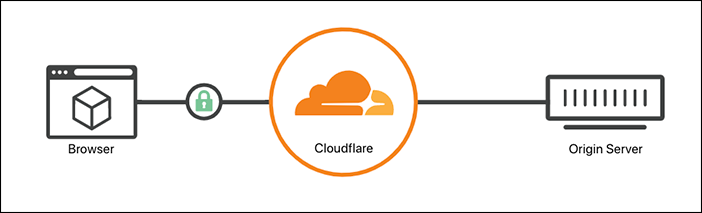
\includegraphics[width=0.8\linewidth]{cloudflare/flexible.png}
    \caption{Cloudflare con configurazione Flexible SSL}%
    \label{fig:flexiblessl}
\end{figure}

L'alternativa alle \emph{Flexible SSL} sono le \emph{Full SSL} (Figura~\ref{fig:fullssl}), queste aggiungono un secondo certificato tra Cloudflare \`e il sito web origine, il certificato pu\`o essere generato da Cloudflare gratuitamente, da Cerfication Authority oppure pu\`o essere generato localmente dall'azienda stessa~\cite{cloudflare-help}.

\begin{figure}[htpb]
    \centering
    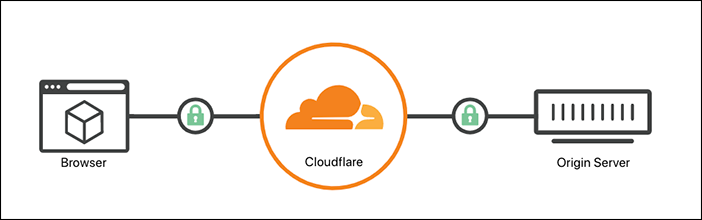
\includegraphics[width=0.8\linewidth]{cloudflare/full.png}
    \caption{Cloudflare con configurazione Full SSL}%
    \label{fig:fullssl}
\end{figure}

L'utilizzo di Full SSL riduce considerevolmente i problemi di sicurezza tuttavia \`e richiesta completa fiducia verso Cloudflare: per permettere di individuare e filtrare i pacchetti malevoli, il traffico tra i visitatori e il server viene decifrato da Cloudflare e poi criptato nuovamente con il secondo certificato. Cloudflare agisce come una VPN ad accesso remoto, il traffico viene cifrato tra il proxy e le sue fonti ma \textbf{il proxy ha accesso completo alle informazioni e pu\`o impersonare ogni utente}. Cloudflare \`e considerato affidabile dalle pi\`u grandi multinazionali del mondo ma questa vulnerabilit\`a potrebbe allontanare i clienti se lo venissero a sapere. Ho deciso di utilizzare la protezione e i certificati Cloudflare esclusivamente nel server web e invece ho deciso di utilizzare un certificato separato per le API\@. In questo modo i dati sono protetti adeguatamente e il sito web \`e protetto da attacchi DDoS\@.
